\documentclass[runningheads]{llncs}
\usepackage[T1]{fontenc}
\usepackage{graphicx}
\begin{document}
\bibliographystyle{splncs04}
\title{Development of Neovim Plugin using Lua and EDA on NYC Crash Data}

\author{Mateusz Gawior}

\institute{University Freiburg, Germany}

\maketitle

\section{Introduction}

Neovim released on November 1, 2015 as a fork of the Vim editor which was
formerly developed in 1991 by Bram Moolenaar with the goal of improving Vim's codebase. 
One of the main points was to maximize extensibility by introducing a new plugin architecture.
Making it easier to develop plugins in any language.

Lua crystallized to be one of the most popular languages for developing plugins for Neovim,
due to it's built-in support, speed and simplicity, making it a perfect starting point for
everyone who wants to dive into the world of Neovim plugin development.

Plugins are a way to extend the functionality of Neovim.
They can be used to add new features which can greatly enhance
the productivity of the user.

MagiSnipp, the plugin which I developed for this paper,
allows the user to manage code snippets inside Neovim.
It is designed to be simple and easy to use, while providing a wide range of features with the aim to enhance the user's productivity while coding.
It is written in Lua and uses the built-in vim API \cite{API} of Neovim to interact with the editor.

In the first part of the paper, I'll talk about the development of MagiSnipp,
mentioning the features, their implementation and potential challenges that came up during development.

For the second part of the paper, I'll use Exploratory Data Analysis (EDA)
to analyze the Motor Vehicle Collisions - Crashes \cite{DATA} dataset.

This involves analyzing the dataset by looking at the structure and content of the data and identifying patterns, anomalies 
and correlation between variables in it. Also cleaning and handling missing data, visualizing the data and
extracting insights to either prove or disprove early assumptions.

The dataset which I will use to conduct EDA, is a public datasets from data.gov \cite{GOV} that contains
information about all police reported Motor Vehicle Crashes in New York City from July 2012 to February 2024.
The dataset is provided by the New York City Police Department (NYPD) and is updated daily.

All reports follow the MV104-AN \cite{MV} template which is required to be filled out when a crash involves an injury,
a death of a person or total property damage of at least 1000 \$.

The goal of the second part of the paper is to use EDA to uncover insights about the dataset and to either prove or disprove early assumptions.

\section{Neovim Plugin Development}

In this section, I'll discuss the development of MagiSnipp. Initially, I'll outline the features and demonstrate their utilization. 
Then, I'll provide in-depth implementation insights into each feature, each with their own dedicated subsection. 
Finally, I'll address the challenges encountered during the development process.

\subsection{Features}

MagiSnipp spans a wide range of features that can be used to manage code snippets efficiently in Neovim.

For one it allows the user to create snippets. Inside Neovim enter visual mode and select
by holding down the left mouse button the range of lines you want to include in the snippet.
Once selected return back to normal mode by hitting the escape key and
save the snippet by pressing the leader and g key combination, by default the leader is backslash. 
You'll then be prompted to input a key mapping for the snippet, which will be used in insert mode to paste the snippet.
Additionally you can provide a name and description for the snippet, which will help identify its purpose inside the mappings 
window and aid in recalling its functionality.

The mappings window can be opened by pressing the leader and o key combination. A floating window on top of the current window will open,
displaying all created snippets. You can navigate through the mappings window by using the arrow keys.
Pressing the enter key on a snippet entry closes the mappings window and opens a new
floating window the snippets window displaying the snippets content. To go back to the mappings window you can press the b key.
To delete a snippet, navigate to the snippet entry in the mappings window and press the d key. To close 
any of the floating windows type :q in the command line.

Finally, to effectively use MagiSnipp, it additionally offers persistence between sessions by saving all snippets in a database file, 
which are retrieved upon the initial usage of the plugin.

\subsection{Creating Snippets}

To be able to create a snippet, I first wrote the get\_selection() function.
This function is called when the user presses the leader and g key combination.
It first grabs the start and end position of the user's visual selection and then tries to retrieve all lines between the start and end position.
If the table that stores the retrieved lines is not empty, indicating that the user selected something,
within the get\_selection() the prompt\_user() function is called.
This function prompts the user to input a key mapping for the snippet, a name and a description.

The only problem is that Neovim internally represents certain key mappings differently than how the user inputs them.
For instance <c-j> or <C-j> becomes <C-J> and " " becomes <Space>. So when attempting to check if the user's mapping <c-j> 
is already occupied within the internal mappings table, it wouldn't be found since it's internally stored as <C-J>. Consequently, 
it could be overwritten, as for Neovim <c-j> and <C-J> are considered the same key mapping.
To ensure that no existing mappings are overwritten I first translated it to its internal representation using a helper function translate\_mapping().

The translate\_mapping() function first creates a throwaway buffer and then sets the user's key mapping specific to that buffer. Consequently storing the mapping inside 
the buffer's internal mappings table.
This ensures that only the mappings assigned to that buffer are altered, leaving those in the user's main buffer intact.
With the user's mapping translated in the throwaway buffer, I can now initiate a API function call 
to that buffer. This call retrieves the internal mappings table as a string, from which I can extract the translated mapping.

Now that the mapping is translated I can ask within prompt\_user() in a loop if the mapping is empty, forbidden or already occupied.
If any of these conditions are met, the user is prompted to enter a different mapping. 
If the mapping is valid, the user is prompted two more times to enter a name and description for the snippet.

If the description exceeds the window's line length, calculated based on the width of the mappings window, the length of the name and mapping, and additional 
separation characters, it is truncated and three dots are added to indicate that the description has been cut off.

To clear the command line from the input prompt I used a API function to send the i<ESC> key sequence to Neovim, 
transitioning it into insert mode and then back to normal mode, effectively clearing the command line from the input text.

Now that prompt\_user() processed the user's input the key mapping, name and description are concatenated into a string and stored with separation 
characters inside snippets\_info.
Moreover, the table containing the retrieved snippet lines is stored based on its mapping inside the snippets\_content table.
Later on, will snippets\_info be used to display the snippets information in the mappings window and snippets\_content will be utilized to 
display the snippets content in the snippets window.

Before the key mapping can be set, the table containing the retrieved lines has to be built into one string using the build\_snippet() function.
This is done, because the API function that maps the key mapping to a action only accepts a function or a string as input.
Hence, I loop over each line, concatenating them into one string followed by a newline character to preserve the form of snippets that span over multiple lines.


\subsection{GUI}
After implementing the create snippet feature, the user needed a way to see the snippets he created. 
For this I implemented a simple GUI that displays all snippets created in a new floating window.

Activated by pressing leader and o the function open\_mappings\_window() first checks
if the snippets window is open and if so it closes it. This prevents multiple windows cluttering the interface. 

Then a API function is called that opens a new floating window on top of the current one with a unique buffer attached to it.
Various options are configured for the mappings window, including setting its width and height to 60 \% of the main window's size,
adding a border, positioning it relative to the main window, inserting a centered title, and applying highlights such as a red border,
blue title and white tint over the current line, enhancing the user's visibility.

The mappings window is now constructed but we still have to fill it with our mappings.
The draw\_mappings\_window() function populates the mappings window.
It accepts a redraw parameter which determines whether to redraw the entire mappings window or to just append the snippets\_info. 
If redraw is true, all lines are cleared from the window's buffer.

If redraw is false, snippets\_info is appended to the mappings window.
To prevent over drawing, snippets\_info is drawn, starting at cached onto the buffer.
After each draw, cached is updated by the number of newly added entries. Before the snippets\_info is emptied all newly added information is stored
inside the cached\_mapp\_win table. Since the index representing the snippet information within cached\_mapp\_win is the same as the index of the snippet
information within the mappings window, it serves as a representation of the mappings window and can be used to redraw the whole mappings window.

Now the user can view the information about the snippets but still needs a way to actually see the snippets content. For this I set up a key mapping in 
the setup() function that upon pressing the enter key inside the buffer of the mappings window calls the snippet\_window() function. 

Based on the the line the user pressed enter on, snippet\_window() first retrieves the content of the current line and searches for " " which always 
follows after a key mapping in the entry of the mappings window, it visually separates it from the other snippet information. 
The index of the space is returned and the substring containing the mapping is cut out and stored in the mapping variable inside snippet\_window().

The snippet window is only created if the mapping is not empty and the previous window is open, and if so closes it. Otherwise there is no content to display.
It is setup the same way as the mappings window, only it draws the content of the snippet stored in snippets\_content. 
To enable quick navigation, specific to the snippets window buffer a key mapping b is set that calls the open\_mappings\_window() function
to be able to return quickly to the mappings window.

\subsection{Deleting Snippets}

I established that the user can create and view his snippets but he also needs a way to delete snippets he no longer needs. 
For this problem I created the delete\_snippet() function. The d key map for it is set in the setup()
function which also only works on the buffer attached to the mappings window.

First it is checked if the mappings window is open and if so the mapping associated with the current line using the
get\_keymap\_from\_line() helper function is retrieved and stored in mapping. If the mapping variable is not empty, indicating 
that the user is not attempting to delete an empty entry, the key map is removed from Neovim's internal table.

Upon deletion it is necessary to update the mappings window to prevent gaps between entries. 
To achieve this the user's current line position is retrieved. 
This line index is then used to remove the corresponding entry from the cached\_mapp\_win table.
The cached\_mapp\_win table now contains all lines besides the one at which the user deleted the snippet.
The gap is now filled, since when you delete a item out of a table all the other items are moved to the left.
To redraw the mappings window cached is set to 0 to ensure that the window is redrawn from the beginning and snippets\_info 
is set to the new representation of the mappings window so to cached\_mapp\_win. 
The mappings window is then redrawn with draw\_mappings\_window(true).

\subsection{Saving snippets}

To ensure seamless management of snippets across sessions, I opted to utilize a database system with the assistance of lsqlite3,
a Lua wrapper around the sqlite3 database engine. I began my importing the lsqlite3 library, storing its return value in the variable sqlite3.

Within db\_create() I used sqlite3 to attempt to open the database, specifying a static path for the root docker.
Once a connection to the database is established, one could execute queries on it.

To enable storage in the database, I first executed a sql query that creates a new table snippets if it 
doesn't already exist yet, with columns mapping, name, description, and snippet.
I chose mapping as the primary key, as I guarantee that every mapping is unique.
After each opened connection and successful query, I closed the connection to conserve resources and avoid potential issues.

The db\_create() function is called within the setup() function, whenever the plugin is first required so loaded into Neovim by the user. 
To make sure that the database is created and ready to store snippets.
In addition to that, if the table already exists the function load\_from\_db() is called.

Inside load\_from\_db() I ran a sql query, that queries all rows of the table. To then loop through each row
and from the columns extract the mapping and snippet to set the key mapping and use mapping, name and description to insert into the snippet\_info table
and store the snippet mapped to the key mapping inside the snippets\_content table.

Storing is performed after a new snippet is created with store\_in\_db().
Which uses a sql query to insert all needed columns into the database table.

\subsection{Challenges}

The main challenge I faced during the development of MagiSnipp was pinpointing the correct functions 
within the Neovim API documentation that would allow me to implement the desired features.
I spent a significant amount of time reading through the documentation and experimenting with different functions 
to determine which ones would be most suitable for my purposes. After rehearsing my code for the paper,
I realized that I could have used nvim\_replace\_termcodes() to translate the user mapping input to its internal representation.

\section{Exploratory Data Analysis}

After concluding the part about the development of MagiSnipp, 
I will now talk about the EDA I conducted on the Motor Vehicle Crashes dataset from NYC. 
First, I'm going to provide a brief overview of the dataset, mentioning the most important 
variables it includes and based on those, I'll come up with some early assumptions. 
Then, I will elaborate on how I cleaned the data and handled missing values. Following that, 
I will discuss how I modified the dataset to obtain the desired answers for my assumptions. 
Subsequently, I will delve into the visualizations and insights extracted from the data. 
Lastly, I will discuss the challenges I faced during the EDA.


\subsection{Overview of the dataset and early assumptions}

The dataset contains a total of 29 columns and about 2.066 million rows as of 20.2.2024, where each row represents a single crash.
The most interesting variables include the id that represents each row uniquely, date and time of the crash, the location of the crash in latitude and longitude, 
the borough and street in which the crash occurred, the number of people injured and killed, the type of vehicles involved and the
contributing factors of each vehicle to the crash.
Based on these variables I formulated following assumptions:
\begin{itemize}
\item The COVID-19 pandemic has led to a decrease in the number of crashes
\item The factors that lead to the most crashes are distraction, speeding and DUI
\item Crash incidents drastically vary between boroughs
\item There are more crash incidents during the day than at night
\end{itemize}

\subsection{Cleaning the data and handling missing values}

Due to the large size of the dataset, it was necessary to first clean and handle missing values.
For cleaning, handling as well as modifying the dataset, I used python with the pandas library.
To gain insight into the amount of missing values, I first read the data into a global pandas dataframe df 
and used isna().sum() to count the missing values for each column, since we do not want to count 
duplicate crashes, I dropped all duplicate rows.

It is evident by looking at the result Table 2 that for the assumption one and four the date and time 
values are all present, and don't need to be handled, still I decided regarding the first assumption to
remove all days of the last month since the month didn't end yet and therefore when plotting the months the data point 
would not be representative for the crashes of the whole month. Furthermore, since for the third assumption 
I want to compare the number of crashes between boroughs, I need to handle the missing values for the borough column.
Since the number of missing values exceeds 642.000 (31 \%) of the data, I decided to deduce the boroughs also 
from the latitude and longitude columns which only is missing about 233.000 values (11 \%) of the data. 

In the worst case I would have 11 \% of the data missing but with the use of
the boroughs column to fill in missing id's that I couldn't deduce from the latitude and longitude columns
this percentage might become even lower which in total is a very good compromise compared to the 31 \%.

By looking at the second assumption, which entails examining various crash contributing factors, 
it becomes evident that many values are absent, particularly for the third, fourth, and fifth factors. 
This observation suggests that most crashes involve no more than two vehicles which entails that they can be safely
disregarded and therefore dropped.

Upon grouping the data by factor, I observed that certain factors exhibit spelling errors or are mentioned ambiguously. 
To rectify this issue, I employed a variations dictionary, which maps incorrect spellings to the correct ones. 
Given the limited number of variations and factors, I undertook the correction process manually to ensure data accuracy.
Additionally I dropped all unspecified factors since they don't provide any useful information.
Other relevant variables, such as the date, time and borough didn't experience outliers and were left untouched.

\subsection{Modifying the dataset}

To analyze my assumptions I first needed to modify the dataset.
The function crashes\_over\_time() was used to analyze the first assumption.
Inside it I first filtered out the date and id column from df and converted the date column to a datetime object.
This conversion allowed me to use datetime functions after setting the date column as an index.

Resample is a datetime method that allows me to group the date by a certain time period,
in this case I used "ME" which stands for month. Upon every grouped month 
I used the count method to count the number of crashes in that month.

For the forth assumption I used the same approach but instead of resampling the date I resampled the time column by hour.

To identify contributing factors for the second assumption I designed the
top\_10\_contributing\_factors() function.
This function first iterates through every column name in df,
identifying those columns that correspond to contributing factors columns.

For every identified factor column, an empty dataframe is instantiated and added to the dfs list.
This step allows me to loop over this list and allocate each dataframe the respective factor column name
based on its index since all factor columns share the same name besides the number at the end.
To later count the number of crashes I also incorporated the id column into each dataframe.

Now I ensured that I have every possible factor with its collision id in a separate dataframe.
To consolidate all dataframes into one to count the number of crashes based on possible factors, 
I standardized the factor column names to ensure compatibility and unionized all dataframes into one.
Following this I utilized groupby to aggregate the data by factor employing count
to count the number of crashes for each factor.

To deal with the third assumption, I created the boroughs\_by\_crashes() function.
It first filters df for the latitude, longitude and collision id columns and stores 
the resulting dataframe in a new variable crashes, also it drops all missing values
since both the latitude and longitude values are needed to deduce the borough. Then to be able to use the latitude and longitude
I first had to convert them to a Point object, I made a lambda function that takes the latitude and longitude as arguments
and returns a Point object with the help of the shapely library. I applied this function on all rows of the 
crashes dataframe using the apply method and stored the result in a new column called geometry.
After filtering out the not anymore needed latitude and longitude columns I created a geodataframe with the help of the
geopandas library out of the crashes dataframe.

Geodataframes are a special type of dataframe that additionally add a geometry column to the dataframe which is used to store spatial data
like Points and Polygons and perform spatial operations with other geodataframes using a common CRS. 

Coordinate reference systems provide a standardized way of describing locations on the surface of Earth.
The epsg:4326 crs is the most common one and is used to represent the earth's surface in latitude and longitude which 
is also used by the dataset.

To deduce the boroughs based on the Point objects, I imported the nybb geodataframe from geopandas.datasets.
It consist of 5 rows where each row includes a borough name from NYC with a geometry column that contains the shape of the borough.
The shape of the borough is represented as a Polygon object and can be used to check if a Point object is within the Polygon object.

Before conducting the spatial join, it was important to ensure that both geodataframes share the same CRS.
The nybb geodataframe utilized the epsg:2263 crs, which is a projected coordinate reference system with feet as the unit of measure.
To ensure compatibility, I converted the CRS of the crashes geodataframe to the espg:2263 CRS with the to\_crs method.
This was necessary because epsg:4326 employs angular units, which are incompatible for direct spatial operations with the projected epsg:2263 CRS.

Finally I conducted the inner spatial join with the sjoin method, which joins the crashes geodataframe with the nybb geodataframe 
based on the geometry column so the location of the crashes and the shape of the boroughs, if a point is within a polygon the row 
is included in the result dataframe if not it is dropped.

The result table crashes\_sj\_nyc includes now the boroughs deduced from the location of the crashes.
Since I only need the boroughs and the collision id's I filtered the result table for those two columns.

I want to also include the boroughs I couldn't deduce from the latitude and longitude columns.
For this I filtered for the boroughs and id column from df and stored the result in a new dataframe boroughs\_id.
I dropped any missing boroughs and extracted using the isin method the id's that are not in the crashes\_sj\_nyc but in boroughs\_id into 
the "missing" dataframe which were about 40 thousand id's.

After aligning the columns of the "missing" dataframe to match those 
in the crashes\_sj\_nyc dataframe, I concatenated both dataframes into a single one to incorporate the missing borough id pairs. 
Finally, I grouped the combined dataframe by borough and used count to determine the total the crash counts.

\subsection{Visualizations and insights}

The final step after modifying the dataset involved visualizing the data using matplotlib, extracting insights from it to either
confirm or disprove the validity of the early assumptions.

For the first assumption, I created a line plot as seen in Figure 3 that visualizes the total number of crashes per month from July 2012 to January 2024.
To enhance the visibility of the individual months, I layered a scatter plot atop the line plot.
The line plot revealed a significant decrease in the number of crashes in 2020, which aligns with the assumption 
that the Coronavirus pandemic led to a decrease in the number of crashes.

What is interesting is that the even years after the start of the pandemic the numbers didn't recover to the level of the years before 2020. 
This could be due to the fact that many companies have switched to remote work and people are not driving as much to work as before.

Additional information that can be inferred is that starting from July 2012, there was a slight rise in monthly crashes, reaching its peak in June 2017. 
It is noteworthy, that between 2016 and 2018, the number of crashes remained relatively stable, but decreased slightly in 2019.
Moreover it can be clearly seen that the nearly for each year the months that produce the most crashes are May and June which could be due to the fact that
the weather is getting better and people are more likely to make trips with the car, also tourists like to travel when it gets warmer maybe influencing the data.
February induces by far the least amount of crashes which could be due to the fact that it is the shortest month of the year.

For the second assumption, I created a horizontal bar plot as seen in Figure 1 that visualizes the top 10 contributing factors to crashes.
The bar plot revealed that the top three contributing factors to crashes are distraction/inattention, failure to yield right-of-way, and following too closely.
Surprisingly, speeding and DUI are not among the top ten contributing factors, which disproves the assumption that these factors lead to the most crashes.
This could be due to that fact that over 2 million factors were noted as unspecified falsifying the data.

For the third assumption, I created a choropleth map as seen in Figure 2 that visualizes the number of crashes in each borough.
The map revealed that indeed crash incidents vary between boroughs, with Brooklyn having the highest number of crashes, 
followed by Queens, Manhattan, Bronx and Staten Island. As expected this correlates with the population of the boroughs,
since Brooklyn is the most populous borough it also has the most crashes and Staten Island the least populous has the least crashes.

For the fourth assumption, I created a line plot as seen in Figure 4 that visualizes the number of crashes per hour which also was overlaid with a scatter plot to see the 
individual hours. The line plot revealed that the most crashes occur between 4 and 5 pm and the fewest between 22 pm to 7 am with the first spike at 8 am confirming the assumption.

All this information infers that most crashes happen when people drive home from work and when people drive to work,
which correlates with the first line plot since it also showed that when people switched to remote work the number of crashes decreased,
indicating that most crashes were caused due to people driving to and from work home.

\subsection{Challenges}

The hardest part of the EDA was to clean the data and handle the missing values. 
I also wanted to look at the type of vehicles involved in the crashes but the data was too messy, with thousands of spelling mistakes and ambiguous words.
I couldn't find a way to clean it properly, I tried to use methods like levenshtein distance to find the most similar words but they didn't work out.

\section{Conclusion}

In summary, the EDA performed on the Motor Vehicle Crashes dataset from NYC has uncovered several noteworthy discoveries. 
Firstly, it showed the importance of cleaning and managing missing data, particularly when dealing with large datasets, 
to ensure the credibility of the obtained results as seen by the missing borough values. Where it was necessary to additionally deduct by location. 
Further, the EDA unveiled these significant findings: the COVID-19 pandemic contributed to a decline in the occurrence of crashes due to the switch to remote work,
driver distraction/inattention is one of the leading contributing factors the lead to crashes, population correlates with number of crashes 
and most crashes happen when people drive to and from work. These findings can be put forward, to encourage companies wherever feasible, to employ remote work for their employees, 
mitigating the risk of future potential crashes.

After utilizing MagiSnipp for a period of time, it's evident that the plugin proves 
beneficial in optimizing code-writing efficiency. By storing frequently used functions as snippets, 
it significantly diminishes the time required for coding tasks, allowing for their quick insertion via a single key mapping.
The user interfaces proves to be intuitive and user-friendly, providing a seamless experience for the user while managing snippets.
Nonetheless, the development of MagiSnipp was not without its challenges, particularly in pinpointing the correct functions within the Neovim API documentation.
Further improvements to the plugin could include the addition of a search feature to the mappings window and replacing the translation function with 
the more efficient nvim\_replace\_termcodes() API function.

\newpage
\begin{thebibliography}{8}

\bibitem{API}
https://neovim.io/doc/user/api (Accessed: 20.02.2024)

\bibitem{DATA}
https://catalog.data.gov/dataset/motor-vehicle-collisions-crashes \newline (Accessed: 20.02.2024)

\bibitem{GOV}
https://data.gov/ (Accessed: 20.02.2024)

\bibitem{MV}

https://www.nhtsa.gov/sites/nhtsa.dot.gov/files/documents/ny\_overlay\_mv-104an\_rev05\_2004.pdf (Accessed: 20.02.2024)

\end{thebibliography}

\begin{table}
    \section{Appendix A: Missing Values}
\center
\caption{All missing values of the dataset}
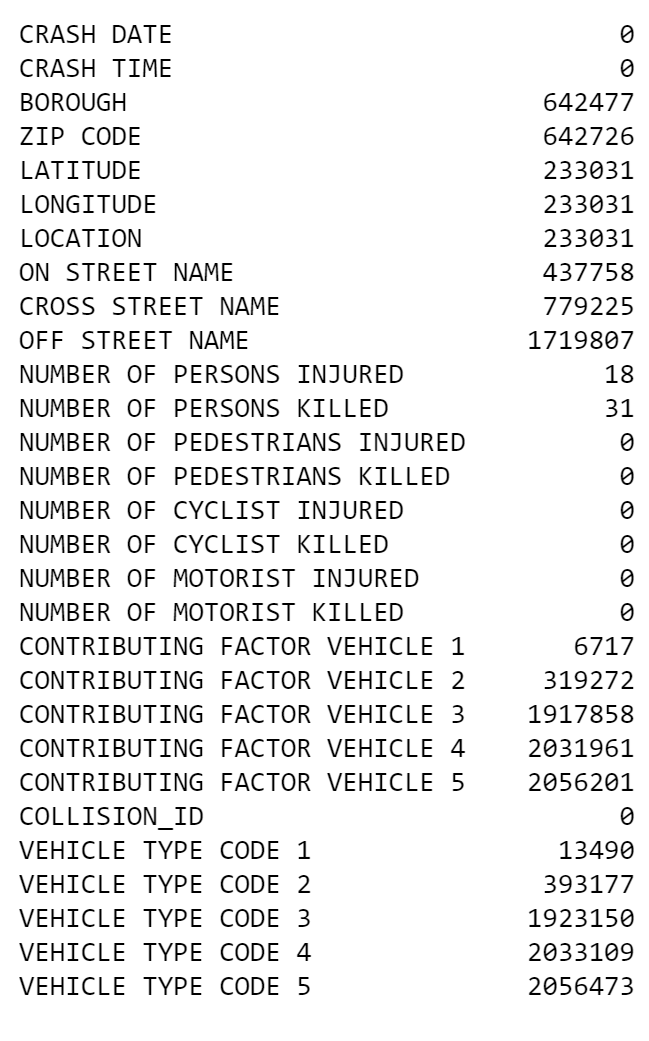
\includegraphics[width=8cm]{datavalues.png}
\end{table}


\begin{figure}
    \section{Appendix B: Plots}
\center
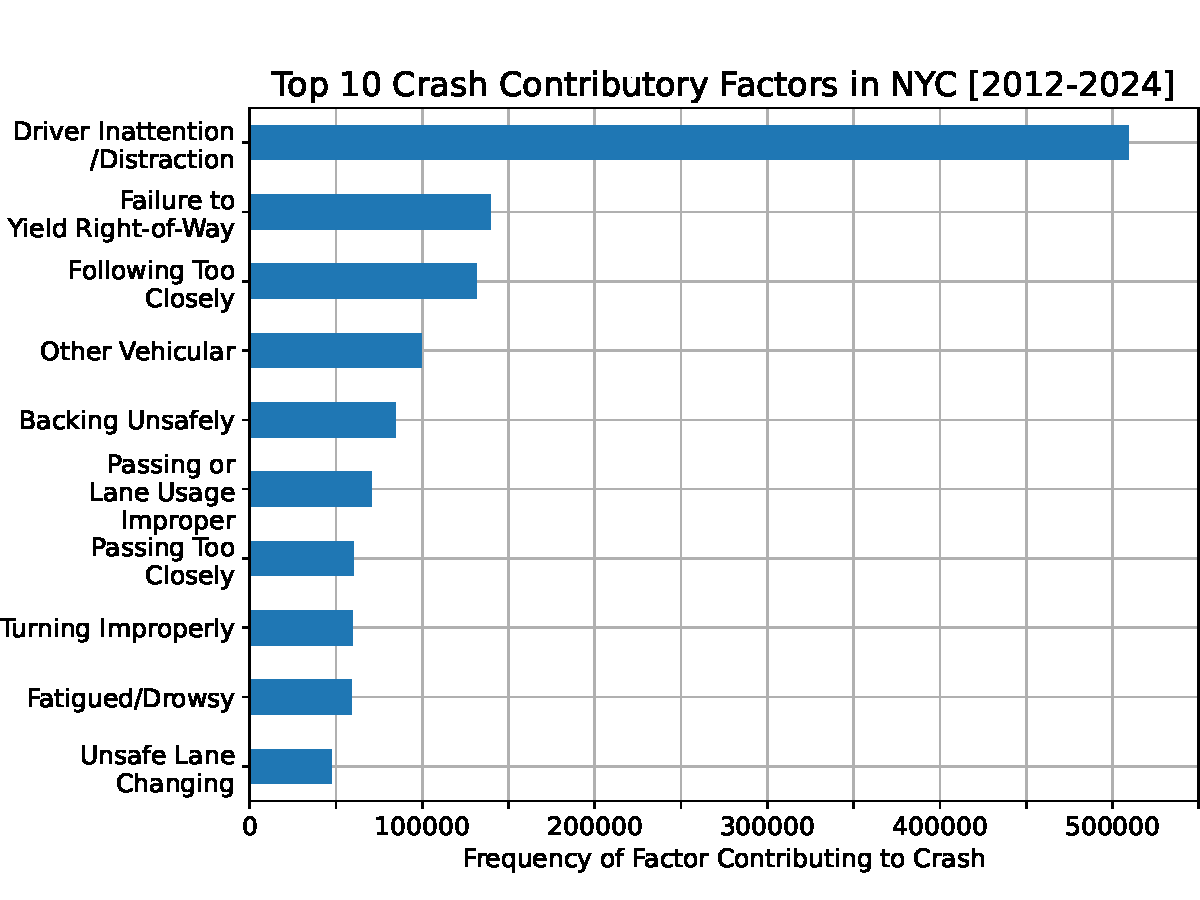
\includegraphics[width=10cm]{top10factors.pdf}
\caption{Top 10 contributing factors to crashes from July 2012 to February 2024}

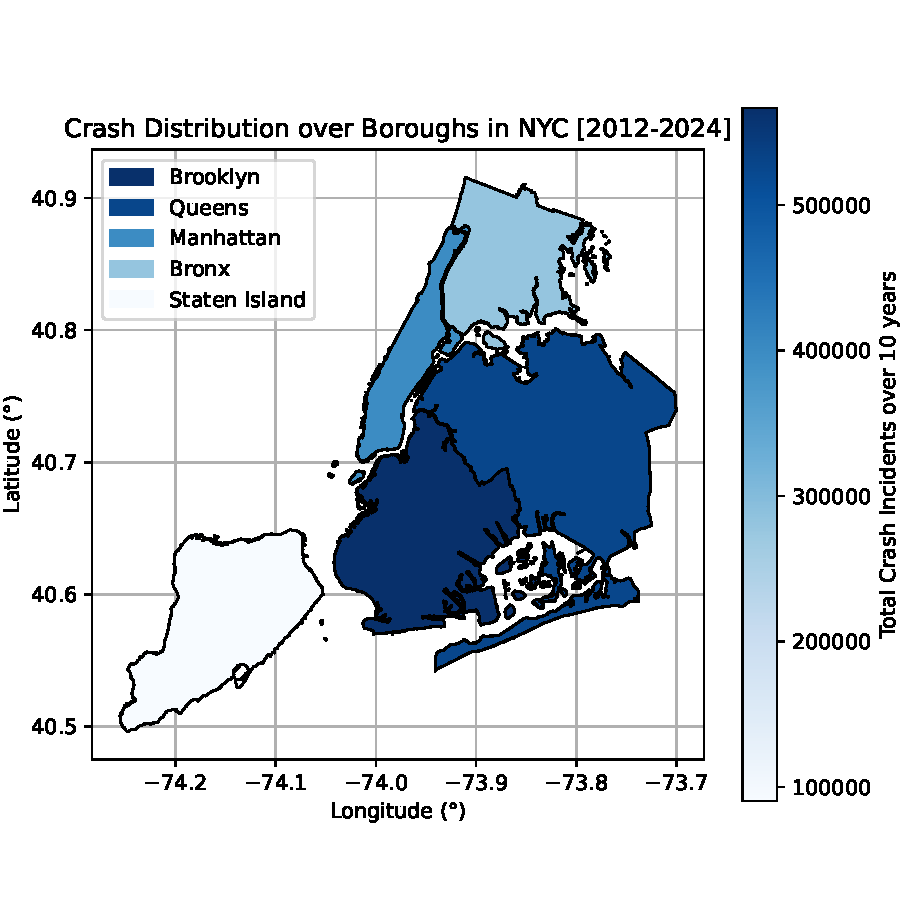
\includegraphics[width=10cm]{boroughsdistr.pdf}
\caption{Total crash distribution by borough from July 2012 to February 2024}
\end{figure}

\begin{figure}
\center
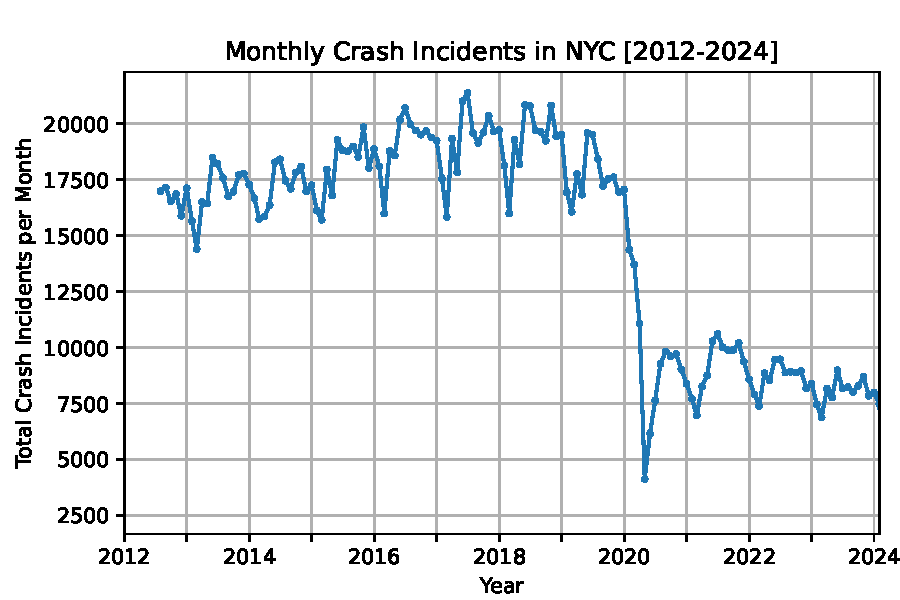
\includegraphics[width=10cm]{crashes_over_year.pdf}
\caption{Total crashes per month from July 2012 to January 2024}

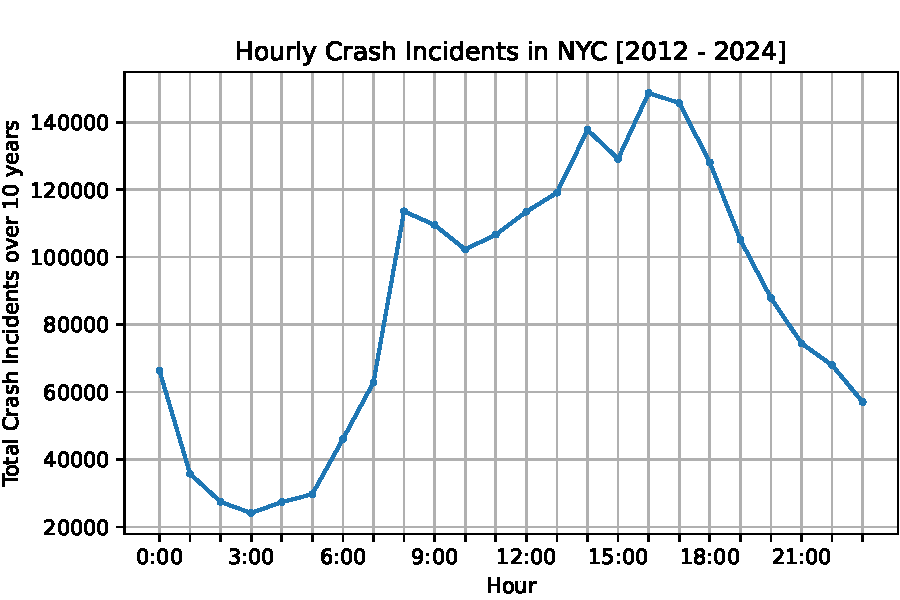
\includegraphics[width=10cm]{crash_by_time.pdf}
\caption{Total crashes per hour from July 2012 to February 2024}
\end{figure}

\begin{table}
    \centering
    \caption{Topics from the lecture}
    \begin{tabular}{c p{6cm}}
        Topics\\
        \hline
        Linux & The EDA as well as the plugin was done under Linux, nothing more. \\
        Text Editor & The paper was written in VSCode, the plugin as well as the EDA was done under Neovim. \\
        Git & Git was used as a repository, nothing more.\\
        Docker & Docker was used to test the plugin, nothing more.\\
        Automation & The EDA was written in python.\\
        Gnuplot & Not used.\\
        \LaTeX & This paper was written in \LaTeX, nothing more.\\
        LLM & Not used.\\
    \end{tabular}
\end{table}

\end{document}